
\documentclass{article}
\usepackage{../HBSuerDemir}\pagestyle{empty}




\begin{document}
\hPage{b1p2/415} 



and having slope y'(0) = Ch 0 = 1 at the origin. From its oddness the graph

is symmetric with respect to the origin. Since Csch x = $\frac {1}{Sh x} $ , the graph

of Csch x is obtained by taking the reciprocals of the ordinates of Sh x.

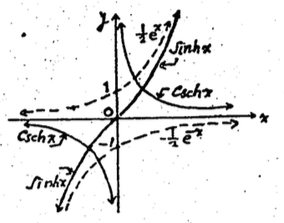
\includegraphics[width=0.65\textwidth,height=0.25\textheight]{images/Graph}

\begin{equation}
   y  = Cosh {x }=  \frac {e^x + e^{-x}}{2}  = \frac {1} {2} e^x + \frac {1}{2} e^{-x} 
\end{equation}
%Equation ba?lat?nca 0.1 gibi bir e?itlik �?k?yor. e?er equation silip ba??na ve sonuna dolar koyarsam da 0.1 e?itli?i siliniyor fakat equation environment ?n? kullanmak do?ru oldu?unu, hspace do?ru olmad???n? s�ylediniz. Umar?m puan k?rmazs?n?z.

This time the curves y = $ \frac {1} {2} e^x $   and   y = $ \frac {1} {2} e^{-x} $  which are symmetric 

with respect to y-axis, are curvilinear  asympotes.

\begin{equation}
y' = Sh x =  \frac {e^x - e^{-x}}{2} = \frac{e^{2x} - T}{2e^x} \Rightarrow e^{2x}=1 \Rightarrow x=0
\end{equation}
%�stteki ayn? a�?klama, equation i�in burada da ge�erli.

The function has critical point at the origin and increasing (decreasing) 
 
when $x>0$  ($x<0$).

The graphs of  Cosh x and Sech x (= 1/cosh x)  are shown in the Fig. 

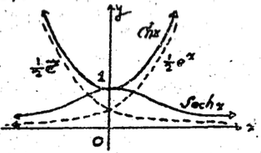
\includegraphics[width=0.65\textwidth,height=0.25\textheight]{images/Graph2}

\begin{equation}
y = Tanh  x= \frac {e^x - e^{-x}}{e^x + e^{-x}}
\end{equation}

It is an odd function. We draw the curve for $x > 0$ and complete the curve 

by symmetry with respect to the origin. \\

 The curve is increasing since $y' = {\operatorname{sech}^2}x > 0 $  and has slope 1 at the origin.

\end{document}













